\chapter{微积分}
\label{chap:calculus}
微积分(Calcuus)是数学的一个基础学科,包括极限、微分学、积分学及其应用。
与机器学习相关的微积分问题有:极值问题、偏导数和梯度。
在机器学习中,定义的所谓模型就是一个包含参数和特征的函数。
定义如下:
$$h_{\theta}(x)=\theta_0+\theta_1x_1+\theta_2x_2+\theta_3x_3+\dots+\theta_nx_n$$
其中,$\theta_i$称为参数,而$x_i$称为特征,$h_{\theta}$是预测模型。
训练模型之前,都会采集很多组样本数据$(x_1, x_2, \dots, x_n)$,
$x_i$就是预设的特征。
模型的准确性,取决于特征的完备性和数据的充分性。
取什么样的特征(采集什么样的数据)有时候也很难确定,过少的或过多的特征,都影响模型的准确性。

\begin{figure}[!htb]
	\centerline{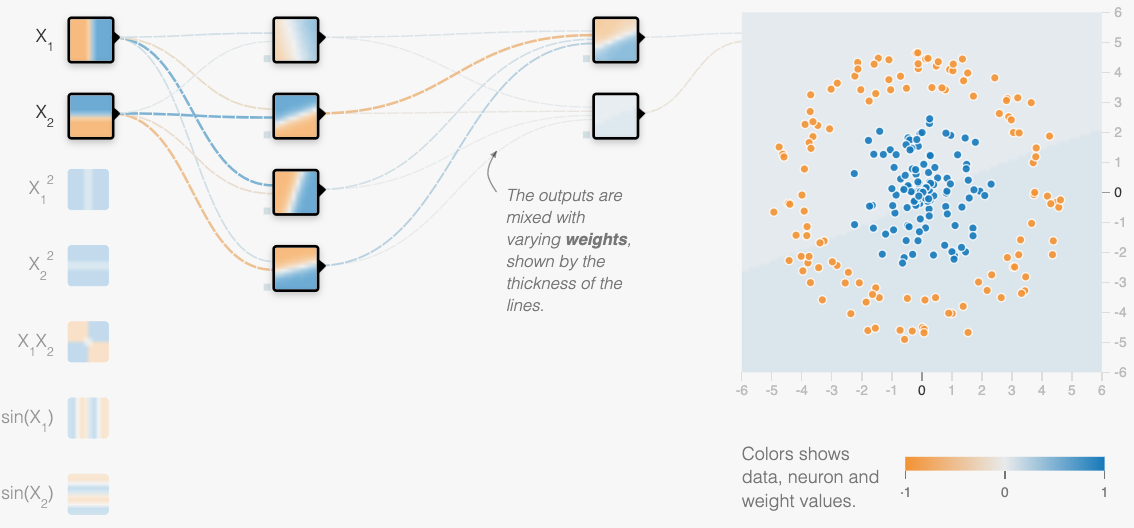
\includegraphics[width=.50\figwidth]{images/x1x2relu.png}}
	\caption{线性特征分类}
	\label{fig:part2_math_x1x2relu}
\end{figure}

极端情况下,已有的样本数据少于特征的维度(相当于未知数多于方程个数),需要引入$\lambda$正则项。
通过\emph{岭回归}(Ridge Regression)得出最优的$\lambda$和$\theta$,下一章线性代数部分会详细说明。

如果特征值$(x_1, x_2, \dots, x_n)$向量线性相关,就有必要减少特征的维度。
很显然,特征空间的维度降低可以极大地简化模型。
采集的样本数据通常都有一些噪点,要引入正则化降低它们对训练结果的影响,防止\emph{过拟合}的出现。
注意,\emph{欠拟合}是指模型包含的特征维度低于现实情况,也无法训练出有效的结果。

由\figref{fig:part2_math_x1x2relu}可知,两个线性特征x1和x2通过线性组合只能训练出多边形特征的模型。
加入特征x3并定义为$x_1^2$,特征x4定义为$x_2^2$,改进后的模型分类预测更符合预期。
实际上,需要哪些特征也并不是那么很明显。首先是我们能获取到哪些数据,主观判断是否相关。
譬如,你可以拿到的数据:(年龄,性别,身高,体重,籍贯),想用于预测某人的籍贯。
$$f(\text{年龄,性别,身高,体重}) -> \text{籍贯}$$

在定义模型之后,通常使用最小二乘法定义\emph{损失函数}(代价函数,Cost Function)。
然后把准备好的大量样本喂给模型,进行迭代训练使其学习出最优的$\vec{\theta}$,
使得代价函数的值尽量小。

$$J(\theta_0, \theta_1, \dots, \theta_n) = \frac{1}{2m}\sum_{i=1}^m(y^i-h_\theta(x^i))^2$$

在机器学习中,使用激活函数对结果进行逻辑分类:
Sigmoid函数,
Tanh函数,
ReLu函数。
它们的主要区别是什么?请同学们仔细观察函数图形之间的共性和区别。

\begin{figure}[!htbp]
\centering
\begin{minipage}{0.33\textwidth}
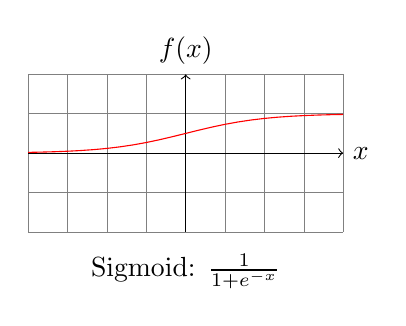
\begin{tikzpicture}[scale=0.5]
  \draw[very thin,color=gray] (-4,-2) grid (4,2);
  \draw[->] (-4,0) -- (4,0) node[right] {$x$};
  \draw[->] (0,-2) -- (0,2) node[above] {$f(x)$};
	\draw[color=red, domain=-4:4] plot (\x,{1/(1+e^-\x)});
	\node at (0, -3) {Sigmoid: $\frac{1}{1+e^{-x}}$};
\end{tikzpicture}
\end{minipage}%
\begin{minipage}{0.33\textwidth}
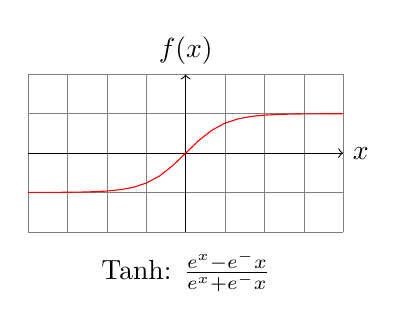
\begin{tikzpicture}[scale=0.5]
  \draw[very thin,color=gray] (-4,-2) grid (4,2);
  \draw[->] (-4,0) -- (4,0) node[right] {$x$};
  \draw[->] (0,-2) -- (0,2) node[above] {$f(x)$};
	\draw[color=red, domain=-4:4] plot (\x,{(e^\x-e^-\x)/(e^\x+e^-\x)});
	\node at (0, -3) {Tanh: $\frac{e^x-e^-x}{e^x+e^-x}$};
\end{tikzpicture}
\end{minipage}%
\begin{minipage}{0.33\textwidth}
	\vspace{0.55cm}
	\begin{tikzpicture}[scale=0.5]
		\draw[very thin,color=gray] (-4,-2) grid (4,2);
		\draw[->] (-4,0) -- (4,0) node[right] {$x$};
		\draw[->] (0,-2) -- (0,2) node[above] {$f(x)$};
		\draw[color=red, domain=-4:0] plot (\x,0);
		\draw[color=red, domain=0:2] plot (\x,\x);
	\node at (0, -3.2) {ReLu: 
			$\begin{cases} 
				x&\text{x>=0}\\0&\text{x<0}
			\end{cases}$};
	\end{tikzpicture}
\end{minipage}%
\end{figure}
引入激活函数不仅用于逻辑分类,关键是还引入了非线性因素。
Sigmoid函数的输出在(0,1)之间,单调连续,并且容易求导。
但它一旦输入落入饱和区,一阶导数就会接近于0,容易产生梯度消失;
Tanh函数也是传统神经网络中常用的激活函数,与Sigmoid一样存在饱和问题。
不过它的输出以0为中心,Tanh函数看上去是放大的Sigmoid函数。

ReLu是目前用的最多也是最受欢迎的激活函数,可加速SGD(梯度下降算法) 的收敛。
但ReLu随着训练的进行,部分输入也会落到硬饱和区。
除了ReLu,还许多ReLu衍生的激活函数,比如:Leaky ReLu、ReLU6、SReLu、PReLu、RReLu、CReLu。


\section{偏导数与梯度}
在微分中,导数表示函数的变化率,也是变化率最大的方向。
梯度是全部偏导数构成的向量,一般将函数$f$的梯度记为$\Delta f$。
根据方向导数的知识,可知梯度的方向即为函数值增长最快的方向。

$$ grad f(x_0, x_1,\cdots, x_n) = (
		\frac{\delta f}{\delta x_0},
		\frac{\delta f}{\delta x_1},
		\cdots,
		\frac{\delta f}{\delta x_n}
) $$

\noindent
函数在某一点的梯度,是一个向量,与最大方向导数的方向一致,
而它的模就是方向导数的最大值。
既然,沿梯度方向具有最大的变化率,所以沿着负梯度方向去减小函数值,
才能最快达到优化目标。

\begin{figure}[!h]
\centering
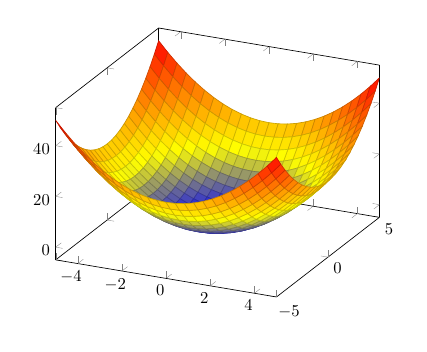
\begin{tikzpicture}[scale=0.6]
	\begin{axis}
	\addplot3[surf]                % 绘制三维图
	 {x^2+y^2};                    % 输入二元显式函数
	\end{axis}
\end{tikzpicture}
\hspace{0.1cm}
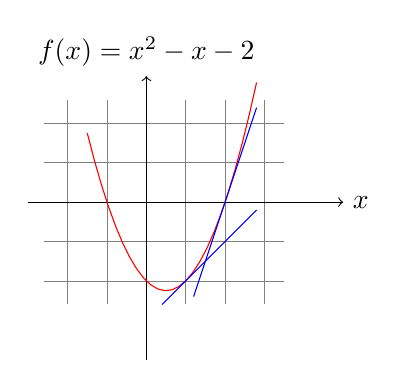
\begin{tikzpicture}[scale=0.5]
  \draw[very thin,color=gray] (-2.6,-2.6) grid (3.5,2.6);
  \draw[->] (-3,0) -- (5,0) node[right] {$x$};
  \draw[->] (0,-4) -- (0,3.2) node[above] {$f(x)=x^2-x-2$};
	\draw[color=red, domain=-1.5:2.8] plot (\x,{\x*\x-\x-2});
	\draw[color=blue, domain=1.2:2.8] plot (\x,{3*\x-6});
	\draw[color=blue, domain=0.4:2.8] plot (\x,{\x-3.0});
\end{tikzpicture}
\end{figure}

\noindent
梯度下降就像是你低头只看脚下的下山过程,若想最快到达山底,
最好每一步都找最陡峭的方向走,这就是梯度的负方向。由于视野的局限性,
使用\emph{梯度下降}也有可能落入局部最小值。

\ \\
\noindent \emph{例子}
	函数 $f(x)=x^2-x-2$, 梯度:$f'(x) = 2x-1$
\begin{lstlisting}[numbers=none]
假设α=0.2可以这样推算: 设起点为(4,0)

1次:参数x=4, 4-0.2*(2*4-1)=2.6
2次:参数x=2.6, 2.6-0.2*(2*2.6-1)= 1.76 
3次:参数x=1.76, 1.76-0.2*(2*1.76-1)=1.256 
4次:参数x=1.256, 1.256-0.2*(2*1.256-1)=0.9536 
5次:参数x=0.9536, 0.9536-0.2*(2*0.9536-1)=0.77216 
......
After 13 steps: x = 0.502743, f(x)= -2.249992. 
After 14 steps: x = 0.501646, f(x)= -2.249997. 
After 15 steps: x = 0.500987, f(x)= -2.249999. 
After 16 steps: x = 0.500592, f(x)= -2.250000. 
After 17 steps: x = 0.500355, f(x)= -2.250000. 
After 18 steps: x = 0.500213, f(x)= -2.250000.
\end{lstlisting}

\section{线性拟合}
样本的散点图有助于发现关键特征,建立正确的模型。
如下图,可直观地识别出线性关系,尽管有干扰数据。
\begin{figure}[!h]
	\begin{center}
	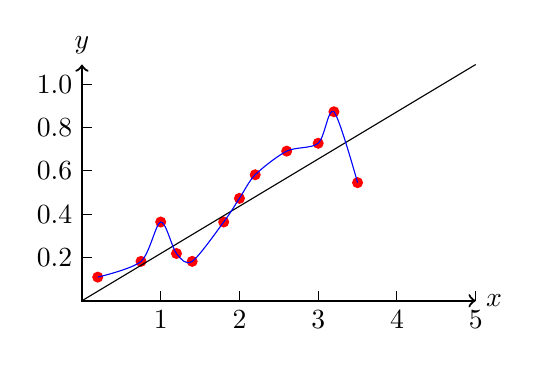
\begin{tikzpicture}
			\pgfmathsetmacro{\ticker}{0.125}
			\draw [<->,thick] (0,3) node (yaxis) [above] {$y$}
							|- (5,0) node (xaxis) [right] {$x$};
			\foreach \i/\texti  in {1,2,3,4,5} {
			\draw (1*\i,0) --(1*\i,\ticker) node[label=below:\texti]{};
			}
			\foreach \j/\textj  in {0.2,0.4,0.6,0.8,1.0} {
			\draw (0,2.75*\j) --(\ticker,2.75*\j) node[label=left:\textj]{};
			}
			\
			\fill[red] (0.2,0.3) circle (2pt);
			\fill[red] (0.75,0.5) circle (2pt);
			\fill[red] (1,1) circle (2pt);
			\fill[red] (1.2,0.6) circle (2pt);
			\fill[red] (1.4,0.5) circle (2pt);
			\fill[red] (1.8,1) circle (2pt);
			\fill[red] (2.0,1.3) circle (2pt);
			\fill[red] (2.2,1.6) circle (2pt);
			\fill[red] (2.6,1.9) circle (2pt);
			\fill[red] (3,2.0) circle (2pt);
			\fill[red] (3.2,2.4) circle (2pt);
			\fill[red] (3.5,1.5) circle (2pt);
			\draw (0,0) -- (5,3) node [] {};
			\draw[blue] plot[smooth] coordinates{
				(0.2,0.3) (0.75,0.5) (1,1) (1.2,0.6) (1.4,0.5)
				(1.8, 1)  (2.0,1.3) (2.2, 1.6) (2.6, 1.9) 
				(3, 2.0) (3.2,2.4) (3.5, 1.5) };
			\end{tikzpicture}
			\caption{线性拟合}
	\end{center}
\end{figure}

拟合指的是你逼近目标函数的远近程度。
\emph{欠拟合},是指模型复杂度过低,不能很好的拟合所有的数据,训练误差大,在训练和预测时表现都不好。
欠拟合很容易被发现,在训练的时候就表现很差。
\emph{过拟合},是指模型复杂度很高,但训练数据很少,导致训练误差小,测试误差也大。
过拟合,过度地学习训练数据中的细节和噪音,以至于模型在新的数据上表现很差,泛化性能变差。
\footnote{欠拟合(underfitting),或者叫作叫做高偏差(bias),过拟合(overfitting),也叫高方差(variance)}

\begin{figure}[!htb]
	\centerline{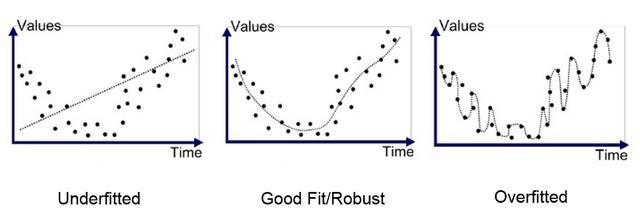
\includegraphics[width=.50\figwidth]{images/overfit_underfit.png}}
	\caption{拟合情况分类}
	\label{fig:part2_math_overfit_underfit}
\end{figure}

\subsection{最小二乘法}
最小二乘法是勒让德( A. M. Legendre)于1805年在其著作《计算慧星轨道的新方法》中提出的。
它的主要思想就是求解未知参数,使得理论值与观测值之差(即误差,或者说残差)的平方和达到最小。

$$E = \sum_{i=1}^n(y_i-\hat{y})\footnote{$y_i$是样本数据,$\hat{y}$是理论值}$$

\section{优化问题}
拉格朗日乘子法(Lagrange Multiplier),用于求解带等式约束的极值问题,而KKT(Karush Kuhn Tucker)条件是拉格朗日乘子法的推广。
在有等式约束时使用拉格朗日乘子法,在有不等约束时使用KKT条件。

\subsection{拉格朗日乘子}
拉格朗日乘子法是一种寻找多元函数在其变量受到一个或多个条件的约束时的极值的方法。
设目标函数为$f(x)$,约束条件为$h_k(x)$,其中s.t. 表示subject to ,“受限于”的意思,$l$表示有$l$个约束条件。
定义如下:

$$L(x,\lambda)=f(x)+\lambda h_k(x)$$
\[
min \enskip f(x) \quad \vert \quad s.t. \enskip h_k(x) = 0 \quad k=1,2,\dots,l
\]

\begin{enumerate} \setlength{\parsep}{0pt} \setlength{\parskip}{0pt}
	\item 构造拉格朗日函数 
	\item 解偏导方程 
	\item 代入上述函数 
\end{enumerate}

由拉格朗日乘子法的定义可知,它是一种寻找极值的方法,因此该方法并不能保证极值点是最低点或者最高点。
\begin{figure}[!htb] \centering 
	\begin{tikzpicture}
		\node at (0,0) {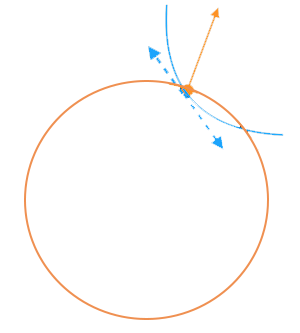
\includegraphics[width=3.5cm]{images/orange-gradient.png}};
		\node at (4,0) {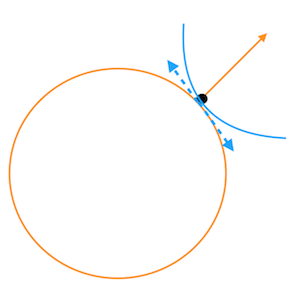
\includegraphics[width=4cm]{images/black-gradient.png}};
		\node at (8,0) {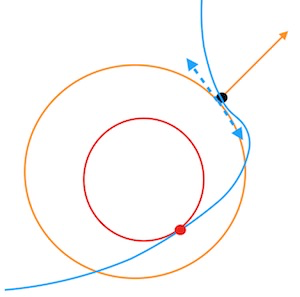
\includegraphics[width=4cm]{images/multiple-solution.png}};
		\node at (0,1.5) {图1};
		\node at (4,1.5) {图2};
		\node at (8,1.5) {图3};
	\end{tikzpicture}
	\caption{拉格朗日算子法}
\end{figure}

这里不加任何推导,很明显相切的时候才能到最低点。
橙线的梯度(上图1橙色箭头)和蓝线的切线(蓝色虚线)不是垂直关系。
蓝线的两个切线方向,分布往函数高处走(与梯度的夹角小于 90 度),和往函数低处走(与梯度的夹角大于 90 度)。
因此,两条曲线相交时,肯定不在最低点或最高点的位置。

如果两条曲线相切(上图2),那么蓝线的切线和橙线的梯度是在切点这个位置垂直。
这时,蓝线的切线方向指向橙线的等高线方向。
图3中相切的点有两个,而红点的明显比黑点小。
要判断找到的点是极低点还是极高点,需要将切点代入原函数再进行判断。
在实际求解时,令各偏导为0就能满是相切的条件。

\subsection{KKT条件}
在优化理论中,KKT条件是非线性规划(Nonlinear Programming)最优解的必要条件。
KKT条件将拉格朗日算子法中的等式约束优化问题推广至不等式约束。
将上一节中的约束等式$h_k(x)=0$推广为$g_i(x) \le 0$,优化问题如下:

\[
	min \enskip f(x) \quad \vert \quad s.t. g(x) \le 0
\]

约束不等式$g(x) \le 0$称为Primal Feasibility,
定义可行域为(Feasible Region)$K=\{x\in\mathbb{R}n∣g(x) \le 0\}$。
设$x^\star$为满足约束条件的最优解,可分为内部解、边界解两种情况。
内部解的时候,$g(x)$不起作用,退化为无约束问题。
边界解的时候,取不等式的边界,约束转换为$g(x)=0$,转化为Lagrange算子法。

\begin{enumerate}
	\item $g(x^\star) \le 0$,最佳解位于K的内部,此时约束条件是无效的;
	\item $g(x^\star)=0$,最佳解落在K的边界,此时约束条件是有效的。
\end{enumerate}

\begin{figure}[!htb] \centering 
	\begin{tikzpicture}
		\node at (0,0.3) {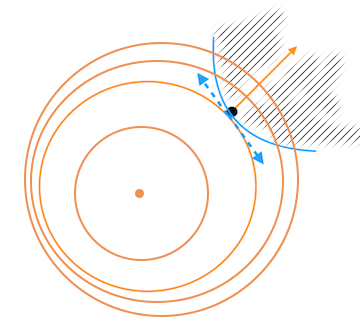
\includegraphics[width=4cm]{images/kkt-region.png}};
		\node at (4,0) {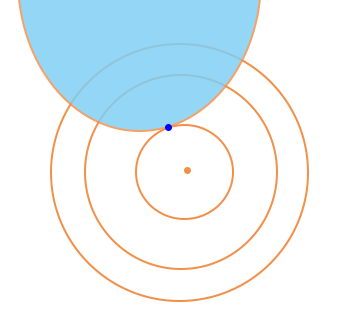
\includegraphics[width=4cm]{images/kkt-cond.png}};
		\node at (8,0) {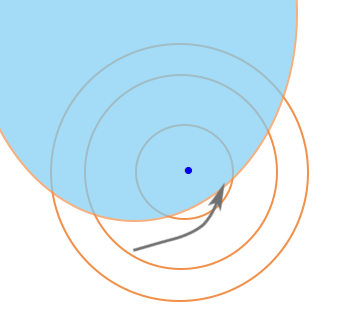
\includegraphics[width=4cm]{images/kkt-cond-2.png}};
		\node at (0,1.5) {图1};
		\node at (4,1.5) {图2};
		\node at (8,1.5) {图3};
		\node at (3.6,0.4) {$x^*$};
		\node at (8,0) {$x^*$};
		\node at (3,0.8) {$g_i(x)=0$};
		\node at (7,-1.3) {$g_i(x)=0$};
	\end{tikzpicture}
	\caption{KKT}
\end{figure}

KKT-图1中,把Lagrange条件变成一个区域,该图的切点处仍旧是最优解。
KKT-图2中,在边界处$g(x)=0$等价于Lagrange算子法。
KKT-图3中,最佳解位于K的内部,约束条件无效。
KKT是SVM(support vector machine)支持向量机的重要理论基础。

\subsection{凸优化}
凸优化在数学规划领域具有非常重要的地位。
若能把一个实际问题表述为凸优化问题,基本上意味着该问题已经得到解决,这是非凸的优化问题所不具有的性质。
机器学习中有很多优化问题都要通过凸优化来求解,即便是在非凸优化中,凸优化同样起着重要的作用。
实际上,很多非凸优化问题,可以转化为凸优化问题来解决。

$$
f_i(\alpha x + \beta y) \le \alpha f_i(x) + \beta f_i(y),
\quad
\text{其中} \alpha + \beta = 1, \alpha \ge 0, \beta \ge 0
$$

\begin{figure}[!htb]
	\centerline{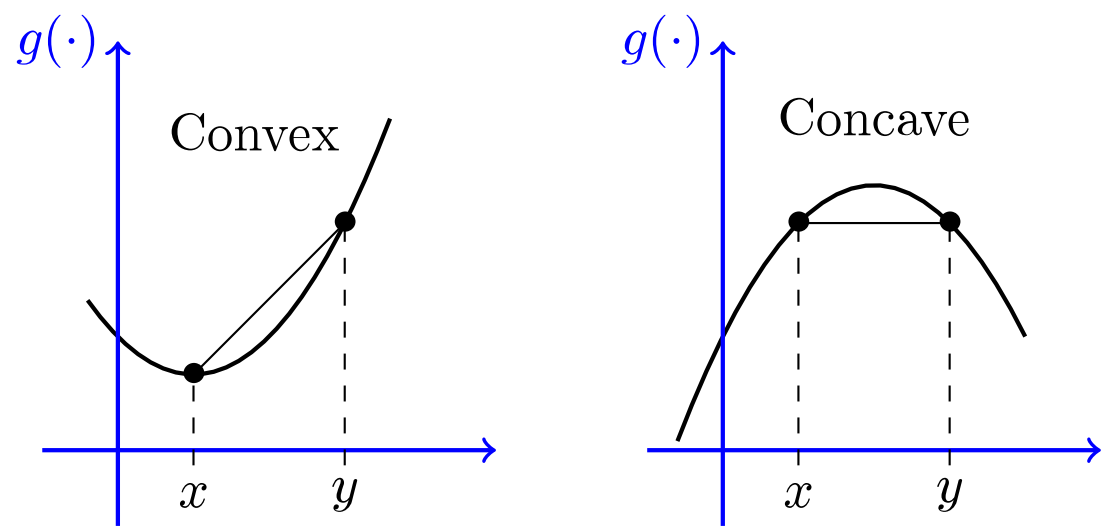
\includegraphics[width=.30\figwidth]{images/convex-concave.png}}
	\caption{凸函数和凹函数}
	\label{fig:part2_math_convex_concave}
\end{figure}

如\figref{fig:part2_math_convex_concave}所示,
凸函数的几何意义为任意两点连线上的取值大于该点在函数上的取值,
而凹函数正好相反。很显然,凸函数总是在其任意一点的切线的上方。
通常使用函数的二阶导来判断一个函数是否为一个凸函数。

$$
\bigtriangledown_x^2f(x) \ge 0
$$

\begin{figure}[!htb]
	\centerline{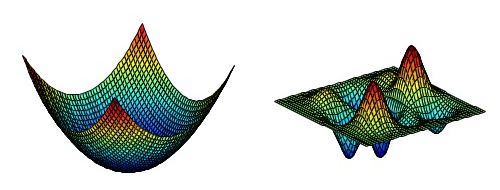
\includegraphics[width=.35\figwidth]{images/concave-to-convex.png}}
	\caption{凹函数转化为多个凸函数优化问题}
	\label{fig:part2_math_concave_to_convex}
\end{figure}

凸优化相对简单,具有良好的几何性质,比如分离平面和支撑平面。
通常凸问题的局部最优解也是全局的最优解,Lagrange对偶是凸优化理论中最重要的工具。
往往只要把某一问题抽象为凸问题,就可近似认为这个问题已经解决了。

SVM本身就是把一个分类问题抽象为凸优化问题,利用凸优化的各种工具(如Lagrange对偶)求解和解释。
深度学习中关键的算法是反向传播(Back Propagation),本质就是凸优化算法中的梯度下降算法。
总的来说,凸优化在工程领域的应用中有着无可撼动的地位。

实际上,生活中几乎所有问题的本质都是非凸的。
如\figref{fig:part2_math_concave_to_convex}所示,
很多非凸问题可以转化成多个凸优化问题,加速问题的求解。

\section{损失函数}
在机器学习中,机器的学习需要某个指标来表示现在的状态,然后,以这个指标为基准,寻找最优权重参数。
机器学习利用已知样本,推演隐藏在背后的真实曲线。这里假设该某曲线为
$h_{\theta}=\theta_0+\theta_1x+\theta_2x^2+\theta_3x^3+\theta_4x^4$ ,
通过样本求解$\theta_i$($i=0\cdots4$)。
不过,这个假设(Hypothesis)很有可能不是最好的。
实际上,我们获得的训练数据总是有误差,不能完全拟合这些数据点,否则就会导致\emph{过拟合}(overfit)的问题。

评价训练过程是否有效,可使用方差衡量源数据和期望值相差的偏离程度。
若是逐渐减小,就是一个有效的训练过程。
这个方差也是一个函数,称为\emph{损失函数}(loss function)\footnote{也称为代价函数(Cost Function)},
用于计算预测值f(x)与真实值y的不一致程度。
它是一个非负的实值函数,通常使用L(Y, f(x))来表示。损失函数值越小,拟合效果就越好。
当样本个数为n时,此时的损失函数变为:
$$
L(Y, f(x)) = \frac{1}{N}\sum\limits_{N}(Y-f(x))^2
$$
$$\text{除2是为了方便求导}$$
$Y-f(X)$表示的是残差,整个式子表示的是残差的平方和,而我们的目的就是最小化残差的平方和。
在实际应用中,通常使用\emph{均方误差}(mean squared error)作为衡量指标,如下:
$$
E=\frac{1}{2} \sum_{k}\left(y_{k}-t_{k}\right)^{2}
$$
在上式中k表示着数据处于哪一个维度,$t_{k}$表示着各维度的监督数据。通常情况下,
监督数据仅将正确解标签表示为1,而其他非正确解则表示为0。
而机器学习输出的结果$y_{k}$,则是会在各个维度都显示该维度是正确解标签的可能性。
均方误差通过计算机器学习的输出和正确解监督数据的各个元素之差的平方,再求总和。
从而得到该权重参数的输出结果与正确结果之间的偏差。

我们现在再介绍另一种常用函数,\emph{交叉熵误差}(cross entropy error)。
其公式如下:
$$
E=-\sum_{k} t_{k} \log y_{k}
$$

在上式中,$y_{k}$代表着机器学习的输出,log表示以e为底数的自然对数($log_{e}$)。
$t_{k}$代表着正确解标签,仅当解标签为正确时,$t_{k}$的索引才为1。其余情况都为0。
因此,E所代表的实际为解标签为正确时所输出的自然对数。


线性回归是确定两个或两个以上变量间关系的一种常见统计分析方法,被广泛用于回归分析。
只有一个自变量的情况称为简单回归,多于一个自变量的情况叫做多元回归。
故可分为一元线性回归分析方程和多元线性回归分析方程。
给定一个随机样本($Y_i, X_i1, \cdots, X_ip$),线性回归模型表示为以下的形式:
$$Y_i = \beta_0+\beta_1X_{i1}+\beta_2X_{i2}+\cdots+\beta_pX_{ip}+\epsilon_i$$
$$i=1,\cdots,n.$$

使用最小二乘法(Least Square Method)需要做矩阵的逆运算,下一章我们再介绍。
而\emph{梯度下降}法起点和学习率都非常重要,顺着梯度$\Delta$下降最快的方向迭代调整。
若干次迭代之后就会落入局部最小点附近,有可能来回震荡无法达到极值点。
所以,调整学习率就非常关键,因此到极值点附近的时候收敛速度也会变慢。




\subsection{反向传播(Back Propgation)}
前述几节,我们利用偏导获得梯度,然后逐步调节参数,朝着误差越来越小的方向迭代。
这还算不上神经元,实际比这还要复杂一些,通常还有一个激活函数(Activation Function),
只有对神经元的刺激足够强才会前向传递。
典型的深度神经网络,至少包含:输入层、隐藏层、输出层。

\begin{figure}[!htb] \centering 
	\begin{tikzpicture}
		\node at (0,0) {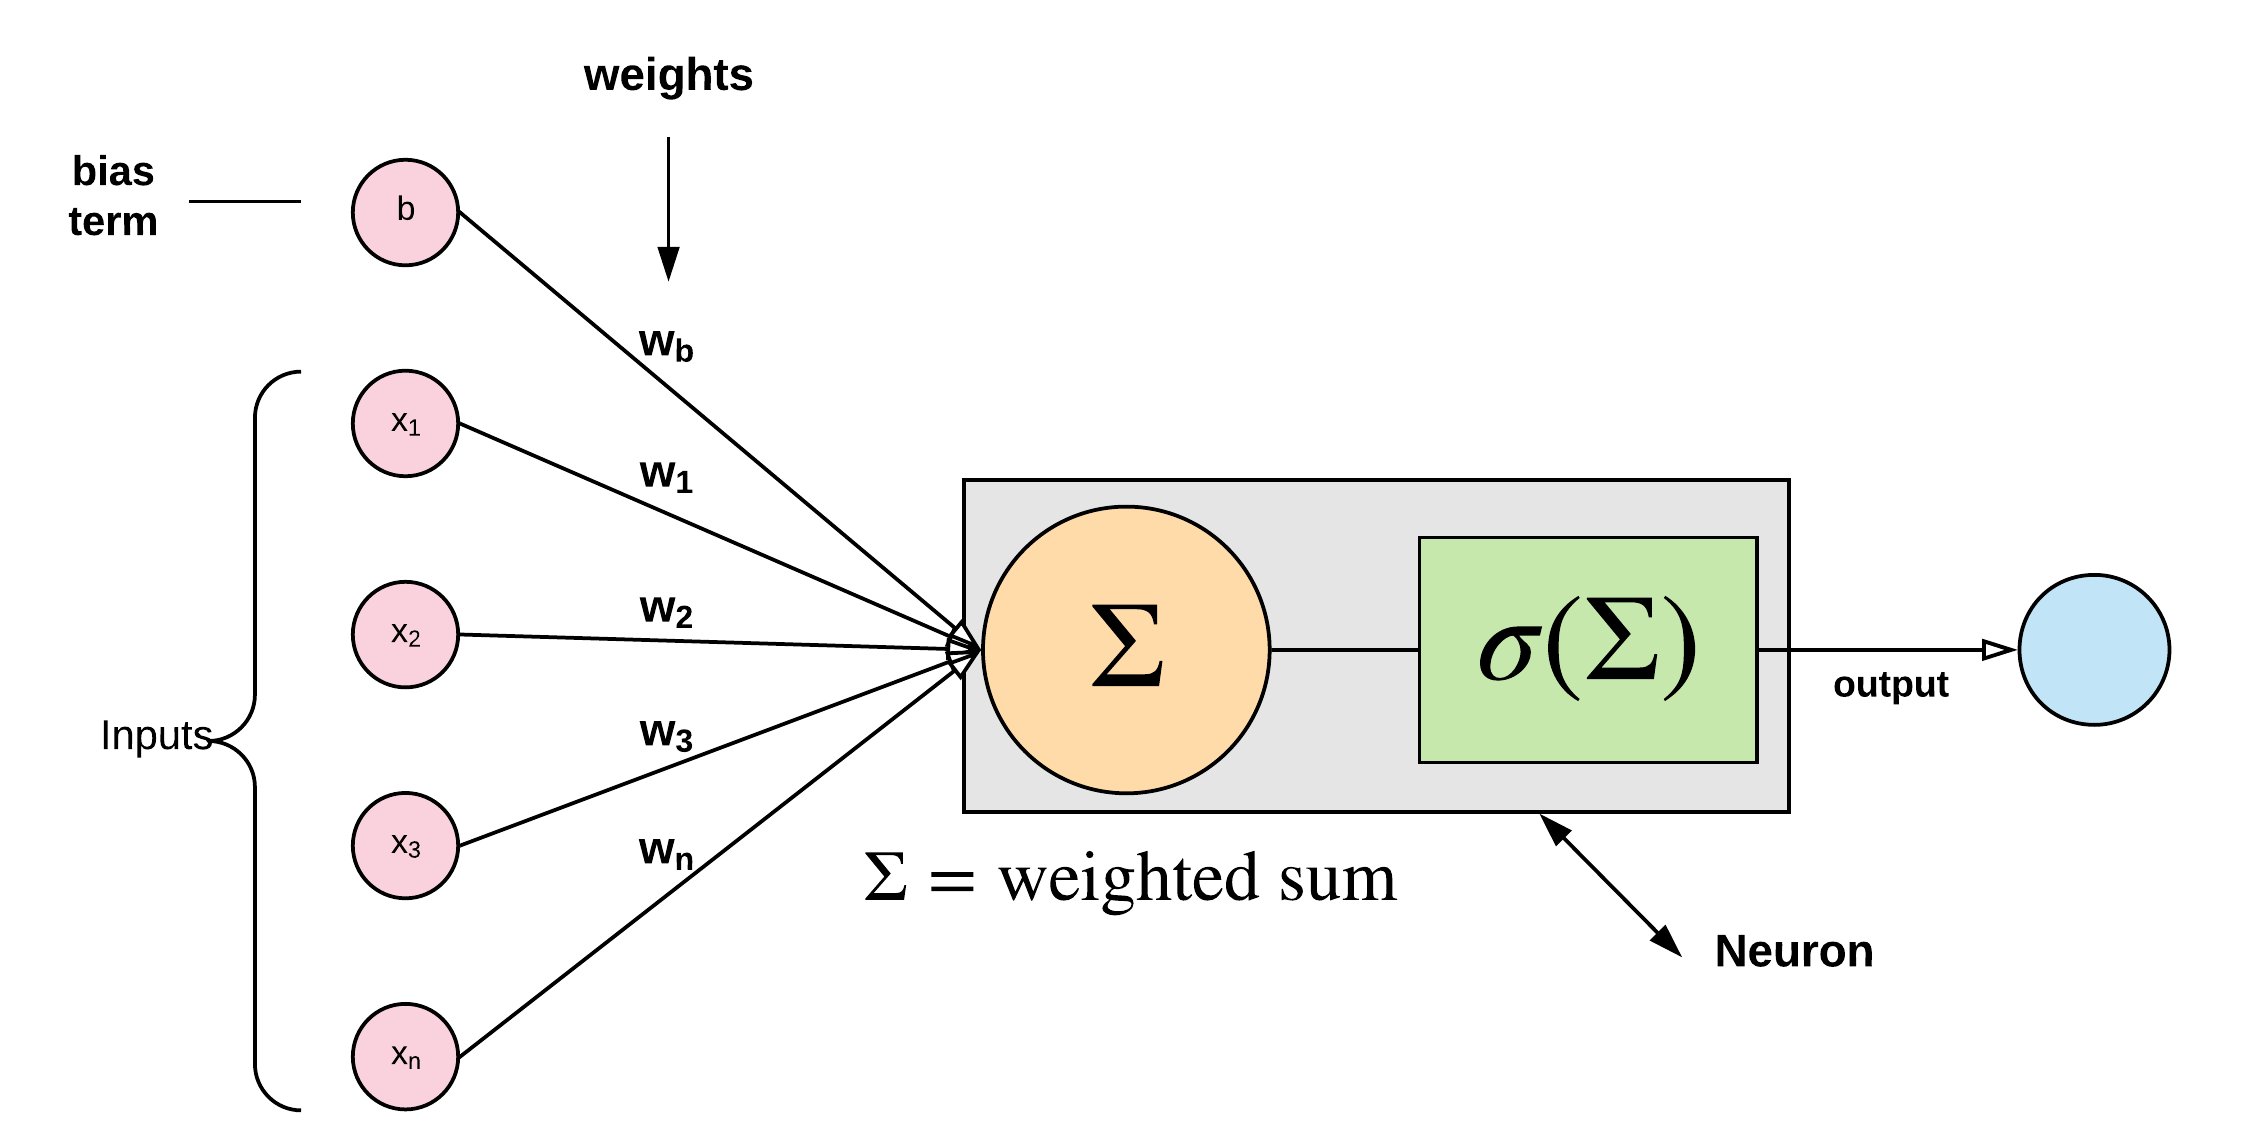
\includegraphics[width=\textwidth]{images/activation-function.png}};
		\node at (1,1) {$\sigma = \text{激活函数}$};
	\end{tikzpicture}
	\caption{神经网络}
	\label{fig:part2_math_neural_node}
\end{figure}

缺少激活函数的线性模型,甚至都无法解决异或问题。
如果选用Linear函数$g(x)=x$作为激活函数就无法划分下图的区域,很显然隐藏层的混入也非常关键。
通过隐藏层引入了更多线段,以便合成一个封闭的多边形,恰好能对数据分类。
激活函数可以在隐藏层引入更多特征,产生非线性结果以解决线性不可分问题。

\begin{figure}[!htb] \centering 
	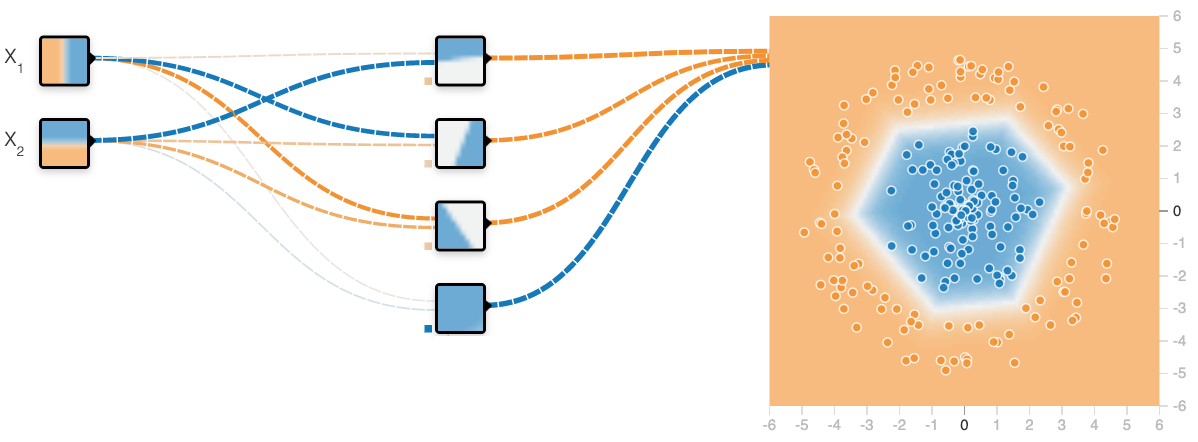
\includegraphics[width=\textwidth]{images/reLu-x1-x2.png}
	\caption{使用激活函数,合成多边形区域}
	\label{fig:part2_math_neural_linear}
\end{figure}


BP神经网络是一种多层的前馈神经网络,分为两个阶段:前向传播和反向传播。
前向传播从输入层经过隐含层,最后到达输出层。
而反向传播从输出层到隐含层,最后到输入层,
逐步调节隐藏层(Hidden Layer)到输出层的权重和偏置(bias),输入层到隐含层的权重和偏置。
经由反向传播,把误差反馈给神经网络用于调节参数。此处不作严格证明,

假设有一个两层深的网络(1个隐藏层),并且每一层只有一个神经元,
$\sigma$为\emph{sigmoid}函数。
相应的数学模型如下:
\begin{figure}[!htb] \centering 
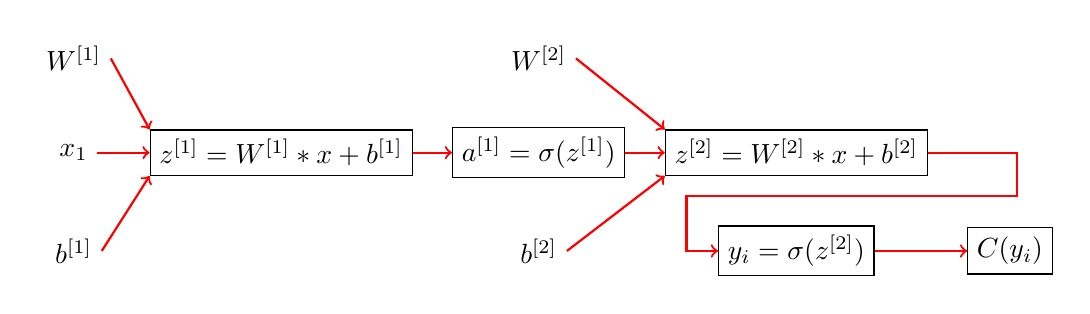
\begin{tikzpicture}
	\matrix [column sep={5mm,between borders}, row sep = 6mm]
	{
		\node (w1) {$W^{[1]}$}; 
			& \node{};
			& \node(w2) {$W^{[2]}$};
			& \node{};
			& \node{}; \\
		
		\node (x1) {$x_1$}; 
			& \node[draw] (n1) {$z^{[1]}=W^{[1]}*x + b^{[1]}$}; 
			& \node[draw] (o1) {$a^{[1]} = \sigma(z^{[1]})$};
			& \node[draw] (n2) {$z^{[2]}=W^{[2]}*x + b^{[2]}$}; 
			& \node{};\\
		
		\node (b1) {$b^{[1]}$}; 
			& \node{}; 
			& \node(b2) {$b^{[2]}$};
			& \node[draw] (o2) {$y_i = \sigma(z^{[2]})$};
			& \node[draw] (C) {$C(y_i)$}; \\
	};
	\draw [->,red,thick] (w1.east) -- (n1.north west) node {};
	\draw [->,red,thick] (x1.east) -- (n1.west) node {};
	\draw [->,red,thick] (b1.east) -- (n1.south west) node {};
	\draw [->,red,thick] (n1.east) -- (o1.west) node {};
	\draw [->,red,thick] (o1.east) -- (n2.west) node {};
	\draw [->,red,thick] (w2.east) -- (n2.north west) node {};
	\draw [->,red,thick] (b2.east) -- (n2.south west) node {};
	\draw [->,red,thick] (n2.east) -| (6,-0.5) -| (1.8, -0.5) |- (o2.west) node {};
	\draw [->,red,thick] (o2.east) -- (C.west) node {};
\end{tikzpicture}
\end{figure}

\noindent
从输入到输出,函数都是平滑的可求偏导的,由误差估计$C(\hat{y})$使用梯度下降法,反向调节参数。
其中, $a^{[i]}$作为下一个神经元的输入,也就是$x_i$。
$$
\frac{\partial{C}}{\partial{b_1}} 
= 
	\frac{\partial{C}}{\partial{y_i}} \cdot
	\frac{\partial{y_i}}{\partial{z_2}} \cdot
	\frac{\partial{z_2}}{\partial{a_1}} \cdot
	\frac{\partial{a_1}}{\partial{z_1}} \cdot
	\frac{\partial{z_1}}{\partial{b_1}}
= 
	\frac{\partial{C}}{\partial{y_i}} \cdot
		\sigma^{'}(z_2) \cdot W_2 \cdot \sigma^{'}(z_1)
$$


如\figref{fig:part2_math_neural_node},
神经网络的输入层就是我们要分类的样本特征,
而隐藏层和输出层每个节点都代表了一个sigmoid单元。
计算的时候,通常把b转化为$x_0$和$w_0$,可把sigmoid单元简化为$net=\sum_{i=0}^nW_ix_i$。
求各输入的和用sigmoid函数得到输出$out=\sigma(net)=\frac{1}{1+e^{-net}}$,
这便是一个单元的计算过程。

整个网络便是前一层作为输入与后一层的每各单元连接,计算出各单元的输出后,再把这一层做为输入传递到后一层。
算法本身并不复杂,隐含在其中的数学推理比较晦涩,包含的过程主要是梯度下降和函数迭代。

